\cotefile{134-2}
\scanpage{170}\mspage{25}
On dira qu'une $n$-catégorie \inserted{$\unsure{\mathcal E|E}_{n}$} est ``\uline{spéciale}'' (ou $n$-\uline{galoisienne}) si elle est $n$-équivalente à la cat. des $(n-1)$-champs loc. constants sur un espace top. (ou un topos) convenable, ou ce qui doit revenir au $\unsure{=|\overline m}$, si elle est $n$-équivalente à la catégorie des $n$-foncteurs $G_n\longrightarrow(n\text{-}\mathrm{Cat})$, où $G_n$ est un $n$-groupoïde. Si $X$, $G_n$, $\mathcal E_n$ se \unsure{correspondent} ainsi, on dit que $\deleted{\unsure{G_n|\mathcal E_n}}\,\unsure{G|\widehat G}_n$ est le $n$-groupoïde fondamental de $X$, ou de $\mathcal E_n$, ou que $\mathcal E_n$ est la catégorie des $n$-systèmes locaux sur $X$, ou sur $G_n$, ou que $X$ est une réalisation géométrique \unsure{de|du} $G_n$ ou de $\mathcal E_n$. En analogie avec le cas bien familier $n=1$, $G_n$ doit s'interpréter comme la sous-$n$-catégorie pleine de $\underline{\mathrm{Hom}}_n(\mathcal E_n,(n\text{-}\mathrm{cat}))$ formée des $n$-foncteurs $\mathcal E_n\to(n\text{-}\mathrm{cat})$ satisfaisant certaines propriétés d'exactitude (on a envie de dire : qui \unsure{commutent} aux $\unsure{\varprojlim|\underline{\lim}}$ finies et aux $\varinjlim$ quelconques) ; mais cela nous attire dans l'inquiétant engrenage des $n$-limites dans les $n$-catégories (\uline{NB} le cas $n=2$ commence à nous être familier\ldots) Il est prudent dans tout
% archive sheet number: 170
\scanpage{171}\mspage{26}
ceci de supposer que $X$ est ``localement homotopiquement trivial'', ce qui assure que le pro-ensemble simplicial que lui associent Artin-Mazur (par le procédé \unsure{de nerfs de|des nerfs de|de nerfs des|des nerfs des} \unsure{'|''}hyperrecouvrements) est essentiellement constant dans la catégorie homotopique ordinaire - donc $X$ définit un type d'homotopie habituel. Ce n'est \uline{pas} le cas bien \unsure{sur|sûr} pour le topos étale d'un schéma. Pour un tel cas, le $n$-groupoïde fondamental doit être conçu comme un \uuline{pro}-$n$-groupoïde (rien d'étonnant à cela, vu la théorie familière \unsure{du|des} $\pi_1$) ; et $\unsure{\mathcal E|E}_n$ comme une $(\mathrm{ind})$-$n$-catégorie (\unsure{la|le} ind-structure correspondant à l'exigence de locale trivialité, pour un $n$-champ variable, relativement à des recouvrements de plus en plus fins de $X$).

\figure{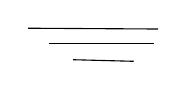
\begin{tikzpicture}[x=1cm,y=1cm]
\draw (0,0)--(1.65,-.01);
\draw (.27,-.19)--(1.60,-.19);
\draw (.57,-.40)--(1.34,-.42);
\end{tikzpicture}}

Je comprends cependant ta résistance instinctive à concevoir ce dépouillement extrême d'un beau topos $X$, au point de n'en retenir que le maigre type d'homotopie. Bien plus, je suis persuadé qu'en
% archive sheet number: 171
\scanpage{172}\mspage{27}
allant jusqu'au bout\unsure{,} de cette résistance à fleur de peau, on arrive à généraliser et à approfondir la notion de ``type d'homotopie'', et à apporter encore une nouvelle eau au développement d'un bon yoga homotopique. Voici où je veux en venir.

Parlons d'abord de faisceaux \inserted{(d'ens., ou de modules \unsure{etc|etc.})}, pour simplifier, au lieu de champs, \inserted{et \unsure{plaçons-nous|plaçons nous} sur le topos étale d'un schéma $X$.} \unsure{Les|les} faisceaux loc. constants - modulo une condition de finitude supplémentaire assez anodine - forment les plus simples des faisceaux \uline{constructibles}, à la définition desquels ils servent de \unsure{modèle|modéle|modele}. Supposant $X$ cohérent ($=$ qu. \unsure{qct|cpct|cpt} et qu. sép), les faisceaux constructibles généraux sont ceux pour lesquels il existe une partition \inserted{finie} $X=\bigcup\limits_{i\in I}X_i$ de $X$ en ``cellules'' \inserted{ou ``strates''} $X_i$, loc. fermées et constructibles, telles que \deleted{\unsure{chaque|chaq.}} la restriction de $F$ à chaque $X_i$ soit \unsure{loc|loc.} constant \deleted{\unsure{et}} (plus une condition de finitude\ldots) Ainsi la catégorie des faisceaux constructibles sur $X$ \unsure{.} (qui redonne la catégorie de tous les faisceaux en passant à une catégorie \unsure{de|des} ind-objets\ldots) \unsure{apparaît|apparait} elle-$\unsure{\overline m|=}$ comme limite inductive de catégories, associées à des partitions de plus en
% archive sheet number: 172
\scanpage{173}\mspage{28}
plus fines de $X$. On peut alors, pour une telle partition \uline{fixée} \inserted{$\unsure{\mathcal P|P}$}, se proposer \unsure{une|d'une} étude approfondie \inserted{de la cat.} des faisceaux (ou complexes de faisceaux, ou champs) qui sont ``$\mathcal P$-constructibles'' (ou plus généralement, qui sont ``loc. constants'' sur chacun des $X_i$). Ces catégories n'auront des \deleted{\unsure{Pour préciser|Pour pouvoir} \unsure{di|de}} \inserted{structures} vraiment satisfaisantes que si elles sont stables par les opérations courantes - telles que $\mathrm R\underline{\mathrm{Hom}}$, ou $\mathrm Rj_*j^*$ où $j:X_i\mathrel{\unsure{-|\longrightarrow}}X$ est une ``cellule'' de la partition, \inserted{etc} . En fait, si $X$ est excellent et qu'on dispose de la résolution des singularités, on sait que les faisceaux \inserted{de torsion} constructibles \unsure{.} (sous réserve d'être premiers aux \unsure{car|car.} résiduelles) sont stables par \deleted{\unsure{toutes}} ces opérations - mais non avec une partition de $X$ fixée une fois pour \unsure{toute|toutes}. Pour avoir une telle stabilité plus fine, il faut faire des hypothèses très strictes \deleted{\unsure{sur}} ``d'équisingularité'' de la stratification donnée de $X$, le long de ses strates. Je pense néanmoins qu'un raffinement des techniques connues \unsure{montrera} que $X$ admet des stratifications arbitrairement fines ayant ces propriétés d'équisingularité (et avec des $X_i$ réguliers et connexes, mais peu importe \unsure{pour} \unsure{notre} propos \unsure{présent}\ldots). \unsure{À|A} titre d'exemple
% archive sheet number: 173
\scanpage{174}\mspage{29}
supposons qu'il y ait exactement deux strates, une strate fermée $X_0$ et $X_1=X-X_0$. D'après le dévissage d'Artin, un faisceau $F$ sur $X$ revient à la donnée d'un faisceau $F_0$ \inserted{$(=i_0^*(F))$} sur $X_0$, d'un faisceau $F_1$ \inserted{$(=i_1^*(F))$} sur $X_1$, et d'un homomorphisme $F_0\longrightarrow i_0^*i_{1*}(F_1)$. Pour que $F$
% Diagram in the left margin, level with "soit".
\margin{\diagram{\resizebox{\linewidth}{!}{\begin{tikzcd}[ampersand replacement=\&,column sep=1.2em]
X_0 \arrow[r,hook,"i_0"] \& X \& X_1 \arrow[l,hook']
\end{tikzcd}}}}%
soit $\unsure{\mathcal P|P}$-constructible, il f et s. que $F_0$ et $F_1$ soient loc. constants (plus des conditions de finitude accessoires\ldots), sur $X_0$ et $X_1$ respectivement. Alors (grâce aux hyp. d'équisingularités) il en sera de $\unsure{\overline m|=}$ de $i_0^*\unsure{i|i'}_{1\unsure{*|,}}(F_1)=\varphi(F_1)$, et \inserted{la cat.} des faisceaux qui nous \unsure{intéressent}\deleted{\unsure{s|t}} s'exprime entièrement en \deleted{\unsure{fonction}} \inserted{termes} de catégories de faisceaux loc. constants sur $X_0$ et $X_1$, \deleted{\uline{\unsure{i.e. de la|i.e. de leurs}} \unsure{d}} \inserted{i.e. des \inserted{seuls} types} d'homotopie de $X_0$ et $X_1$, à celà près qu'il faut encore expliciter la nature du foncteur exact à g. $\varphi$. Je pense que ceci est possible, dans le contexte \inserted{\uline{schématique}} où je me suis placé (techniquement assez sophistiqué), en introduisant un ``voisinage tubulaire étale'' de $X_0$ dans $X$ (qui est un topos fort \unsure{intéressant|satisfaisant}, mais pas associé à un schéma). Mais cette construction technique ne \unsure{fait|fais} que para%
% archive sheet number: 174
\scanpage{175}\mspage{30}%
phraser une intuition topologique extrêmement simple, que je vais expliciter, en supposant pour fixer les idées qu'on est sur le corps de base $\mathbb C$ et qu'on en profite pour travailler avec les espaces loc. compacts habituels. L'idée topologique derrière l'hypothèse d'équisingularité, c'est qu'il existe un \uline{voisinage tubulaire $T$} de $X_0$ dans $X$ se rétractant sur $X_0$, et tel que $(X_0,T)$ au dessus de $X_0$ soit un fibré \unsure{localement|loclement} trivial, donc $T-X_0$ au dessus de $X_0$ est \unsure{loc|loc.|lui} trivial. En fait, \deleted{\unsure{on pourra con|on pourra cons}} \inserted{si $\partial T$ est le} ``bord'' de $T$, qui sera aussi fibré loc. trivial sur $X_0$, $T$ sur $X$ est le fibré en cônes déduit ($\simeq(\partial T\times I)\amalg_{\partial T}X_0$, où $I=[0,1]$, $\partial T\mathrel{\unsure{\to|-}}\partial T\times I$ défini par $x\mathrel{\unsure{\mapsto|\vdash}}(x,1)$, et $\partial T\mathrel{\unsure{-|\to}}X_0$ est la projection) donc $\mathring T=T-X_0\simeq\partial T\times[0,1[$ est $X_0$-homotope à $\partial T$. Si $X_0$ et $X_1$ sont non singuliers, il en est de $\unsure{=|\overline m}$ de $\mathring T$ et $\partial T$, qui sont des fibrés topologiquement lisses sur $X_0$. D'ailleurs, $\deleted{\unsure{X_1|X}}$ posant $\widetilde X_1=X_1-\mathring T$, \deleted{$\unsure{\widetilde X_1|X_1}$ \unsure{dev.}} l'inclusion $\widetilde X_1\hookrightarrow X_1$ est une équivalence d'homotopie, et $X$ se réconstitue, à homéomorphisme près, à partir \unsure{du|des} diagramme d'espaces
\diagram{\begin{tikzcd}[ampersand replacement=\&,column sep=small,row sep=large]
(\mathring T=T-X_0\underline{\approx}) \& \partial T \arrow[r,"\unsure{j|J}","\text{inclusion}"'] \arrow[d,"p","\text{fibration}"'] \& \widetilde X_1\,(\underline{\approx}X_1)\\
\& X_0 \&
\end{tikzcd}}
comme la somme amalgamée. En termes de ce diagramme d'espaces\unsure{;|,} le foncteur $\varphi$ plus
% archive sheet number: 175
\scanpage{176}\mspage{31}
haut s'interprète immédiatement comme
\[
\varphi(F_1)\simeq p_*j^*(\widetilde F_1)
\]
où $F_1\mapsto\widetilde F_1$ est la restriction de $X_1$ à $\widetilde X_1$ (qui est donc une équivalence de catégories pour les faisceaux (loc. const.) envisagés). \deleted{\unsure{Il|Il s'|j} \unsure{peut|peut se|\ensuremath{j^*}}} \inserted{La donnée} d'un\inserted{\unsure{e}} $F=(F_0,F_1,u:\unsure{F|\overline F}_0\to\varphi F_1)$ peut donc aussi s'expliciter comme la donnée de
\[
F_0,\ \widetilde F_1,\ \widetilde u:p^*(F_0)\longrightarrow j^*(\widetilde F_1)
\]
où $F_0$ ($\widetilde F_1$) est un faisceau loc. constant sur $X_0$ (resp. $\widetilde X_1$). Il faut se rappeler de plus \unsure{que ici|qu'ici} $p$ est une vraie fibration, et $j$ une inclusion (et pratiquement, - cas $X_0,X_1$ lisses - \deleted{\unsure{une}} l'inclusion du bord dans une variété à bord).

Si on préfère, on peut aussi prendre le diagramme un peu moins joli (mais un peu plus canonique)
\diagram{\begin{tikzcd}[ampersand replacement=\&,column sep=large,row sep=large]
\mathring T \arrow[r,"\unsure{j|J}'"] \arrow[d,"p'"] \& X_1\\
X_0 \&
\end{tikzcd}}
revenant essentiellement au $\unsure{=|\overline m}$, car formé d'espaces homotopes au précédent. On peut $\overline m$ y remplacer $X_0$ par $T$ ($X_0$ en étant un rétract par déformation) et écrire
\diagram{\begin{tikzcd}[ampersand replacement=\&,column sep=large,row sep=large]
\mathring T \arrow[r,hook,"j'"] \arrow[d,hook,"p''"] \& X_1\\
\unsure{T|I} \&
\end{tikzcd}}
% archive sheet number: 176
\scanpage{177}\mspage{32}
où ``pris à la lettre'' $p''$ est maintenant une inclusion, mais ``moralement'' c'est \inserted{\unsure{tjrs|tjrs.}} une fibration à fibres très \unsure{polies|jolies} [de dim finie notamment, voire des variétés non singulières - c'est donc beaucoup mieux que ce que nous donne le yoga de Cartan-Serre ``toute application continue est équivalente à une fibration''\ldots] C'est ce dernier diagramme qui est susceptible d'une construction directe, purement algébrique, dans le cadre des schémas, lorsque l'on a développé la construction du voisinage tubulaire étale.

Le point où je veux en venir, c'est que la considération \inserted{de la \unsure{cat.|cat}} des faisceaux (ou \inserted{complexes d'iceux, ou} $n$-champs, \unsure{\ldots|..}) $\unsure{\mathcal P|P}$-constructibles sur un $X$, où $\mathcal P$ est une stratification ``équisingulière'' donnée, revient dans le cas particulier actuel à la connaissance d'un diagramme de \uline{types d'homotopie} \inserted{ordinaires} \inserted{(ou de pro-types, si on revient à la top. étale)}
\diagram{\begin{tikzcd}[ampersand replacement=\&,column sep=large,row sep=large]
\unsure{\Delta|\triangle} \arrow[r,"\unsure{j|J}"] \arrow[d,"p"'] \& X_1\\
X_0 \&
\end{tikzcd}}
\unsure{en|et} prenant des systèmes de \unsure{coeff|coeff.} locaux (ou de $n$-champs loc. constants) sur ces sommets \inserted{$X_0,X_1$ \deleted{$\unsure{\Delta|X}$}} reliés par des hom de compatibilité du type $p^*(F_0)\to j^*\unsure{(}F_1)$. Ce serait un exercice amusant (que je n'\unsure{ai} pas encore fait) de
% archive sheet number: 177
